\setcounter{chapter}{2}
\chapter[Regional scale risk analysis accounting for time-dependent vulnerability]{Regional scale risk analysis accounting for time-dependent vulnerability}\label{chap-time}

\begin{small}
This chapter is a published (peer-reviewed) conference paper. 
\\
\\ \noindent
    \textbf{Rabonza, M.L.} and Lallemant, D. (2019). Accounting for time and state-dependent vulnerability of structural systems. \textit{In Proceedings of the 13th International Conference on Applications of Statistics and Probability in Civil Engineering (ICASP13) Sep 2019}. pp. 2298-2305. https://doi.org/10.22725/ICASP13.465
\\
\\
In addition, this chapter cites the following first-author conference paper, which is included in Appendix \ref{app-time-paper}. The paper demonstrates an additional case study, which is an application of the flexible community-scale analysis shown in this chapter. The application focuses on data derived from New Zealand's seismic retrofit implementation records.
\\
\\
\noindent
\textbf{Rabonza, M.L.} and Lallemant, D. (2018). A time-dependent model for seismic risk reduction policy analysis. Accepted in the \textit{17th U.S.-Japan-New Zealand Workshop on the Improvement of Structural Engineering and Resilience Nov 2018. https://hdl.handle.net/10356/164235}

    %%%  Add the ATC paper -- serves as additional case study
% %----------------
% \subsection*{Highlights}
% %--- RESEARCH HIGHLIGHTS
% %----------------
    
% \begin{itemize}
% \setlength\itemsep{-0.45em}

% \item I present a flexible framework to account for time-dependent physical vulnerability in seismic risk analysis.

% \item I model processes that increase vulnerability (deterioration) and policies that mitigate increase in vulnerability (retrofits, maintenance).

% \item I build on the fundamental probabilistic performance based framework by adding a time-varying model for vulnerability.

% \item I provide a tool to study the consequences of seismic mitigation on future seismic risk.

% \end{itemize}


%%% Start of highlights
\clearpage
\vspace*{\fill}
\begingroup
\centering

\textbf{\Large{Chapter highlights}}

\hrulefill 

\begin{itemize}
\item \textsl{I present a flexible framework to account for time-dependent physical vulnerability in seismic risk analysis.}

\item \textsl{I model processes that increase vulnerability (deterioration) and policies that mitigate increase in vulnerability (retrofits, maintenance).}

\item \textsl{I build on the fundamental probabilistic performance based framework by adding a time-varying model for vulnerability.}

\item \textsl{I provide a tool to study the consequences of seismic mitigation on future seismic risk.}
\end{itemize}


\endgroup
\vspace*{\fill}
%%% End of Highlights

%----------------
% \vspace{1cm}
% \noindent
% \textbf{Keywords:} Performance-Based Earthquake Engineering; Risk analysis; Markov chains; Time-dependent risk


\end{small}
\clearpage

%%%%%%%%%%%%%%%%%
\section{Abstract}

The typical process of engineering risk analysis assumes a static state of vulnerability through the lifespan of the structure. However, many civil engineering systems change states over time causing significant impact on their vulnerability. Such dynamic changes may involve an increase in vulnerability driven by deterioration processes (e.g. corrosion, fatigue, creep, hazard-induced damage, etc.), or a decrease in vulnerability driven by strengthening interventions (e.g. retrofitting, maintenance, building replacement, etc.). Accounting for these dynamics is critical to properly understand hazard-related risk of civil engineering systems over their lifespan. This paper presents a stochastic framework for accounting for time and state dependent vulnerability in risk analysis of civil engineering systems. Time-homogeneous Markov chains are used to model various state change processes, and integrated within the risk analysis framework in closed-form expressions. Several applications are demonstrated: (1) quantifying risk of structurally deteriorating buildings and the risk reduction impact of maintenance, (2) urban-scale seismic retrofitting policies based on various retrofit rates, and (3) impact of varying rates of building replacement to higher design grade. These demonstrate the importance of accounting for time dependent state change as a significant factor in the life-span vulnerability of the built environment. The study further provides a framework to study and compare various risk reduction policies.


%%%%%%%%%%%%%%%%%%%%%%%%%%%%%%%%%%%%%%%%%%%%%%%%%%

\section{Introduction}
Developing well-informed and proactive strategies for seismic risk reduction requires the ability to predict risk in constantly changing urban environments, and understand how risk reduction policies affect future seismic risk. However, current seismic risk assessment methods focus on understanding risk to infrastructure in only their present state.

In this paper, we present a flexible framework accounting for time and state dependent vulnerability in seismic risk analysis. This allows for the modelling of processes that can increase vulnerability (e.g. deterioration, building expansions, cumulative damage), those policies that mitigate increase in vulnerability (e.g. better maintenance schedule, higher durability construction) and those policies that improve resilience (e.g. seismic retrofits and building replacement to higher standards).

The framework is applied to hypothetical case studies to demonstrate the effects of time and state dependent vulnerability on a single deteriorating building and to a neighborhood with buildings experiencing deterioration, retrofitting, and building replacements over time. While it is expected that retrofit policies and building replacements lead to decreased seismic risk, and deterioration leads to increased seismic risk over time, this paper demonstrates how risk evolves with time linked to various seismic reduction policies. This methodology is an extension of a time-dependent framework applied to investigate incremental building expansion as the significant driver for increasing risk and vulnerability \citep{lallemant2017framework}.

The key contribution of this paper is to provide a tool for stakeholders to investigate the consequences of various seismic mitigation decisions to future seismic risk. The case study presents a proof of concept and a demonstration rather than actual risk prediction. The framework can be utilized to study a more realistic case once information for transition rates, vulnerability and building stock distribution are available.

\section{Methodology}

\subsection{Proposed framework accounting for time dependent vulnerability in seismic risk analysis}

The Performance-Based Earthquake Engineering (PBEE) methodology proposes a systematic methodology to calculate the seismic risk of structures through the probabilistic integration of (1) seismic hazard, (2) seismic demand, (3) damage capacity, combined into a single impact assessment \citep{krawinkler2004performance}.  Each of these components are described in Table \ref{tab:varlist}. 


\afterpage{%
    \clearpage% Flush earlier floats (otherwise order might not be correct)
    \begin{landscape}% Landscape page
% Please add the following required packages to your document preamble:
% \usepackage{booktabs}
% \begin{tiny}
\begin{table*}[]
\centering
% \footnotesize
\caption{Four components and associated variables of the Performance-Based Earthquake Engineering framework. Descriptions based on explanations by \cite{krawinkler2004performance,deierlein2004overview,moehle2004framework}}
\begin{tabular}{@{}lll@{}}
\toprule
Framework component              & Variable name          & Description of variable                                                                                                       \\ \midrule
Hazard analysis                & Intensity measure (IM)                     & Earthquake induced shaking at study site                                                             \\
Demand analysis      & Engineering demand parameter (EDP)                    & Response of structure to earthquake loading                                                            \\
Damage capacity modelling          & Component damage measure (DM)                     & Seismic-induced damage sustained by  structure                                               \\
Impact assessment                & Decision variable(DV)                     & Performance-related variables for decision making                                             \\ \bottomrule
\end{tabular}
\label{tab:varlist}
\end{table*}
% \end{tiny}
\end{landscape}
\clearpage% Flush page
}

Each step in the probabilistic risk analysis framework comes with inherent uncertainty/variability, thus each associated variable is expressed in the form of conditional probability of exceedance (Figure \ref{fig:schematic1}. With the basic PBEE framework, the final expression for the decision variable, $\lambda_{DV}$,is obtained by combining the conditional probabilities using the total probability theorem. The decision variable then serves as a guide for infrastructure managers to create appropriate risk management and mitigation strategies based on a performance target or risk metric.
\newcommand{\Int}{\int\limits}
\begin{equation}
\begin{split}
    \lambda_{DV} = \Int_{im}^{} \Int_{edp}^{} \Int_{dm}^{} G_{DV|DM}(dv/dm)   \\
    \times \; |dG_{DM|EDP}(dm|edp)|  \\
    \times \; |dG_{EDP|IM}(edp|im)| \nu_{IM}  
\end{split}
\end{equation}

The basic PBEE framework is not capable of dealing with time-dependence of each of the variables, and does not incorporate other potential time-dependent drivers of vulnerability that could affect future seismic risk.
Using the PBEE framework as a starting point, the proposed framework incorporates a new module to account for potential time dependent drivers of vulnerability. 
A similar performance-based framework which accounts for time varying effects of deterioration for bridges was proposed by \cite{rao2017development}. Building on the PBEE methodology and \cite{rao2017development}'s framework, we propose a flexible framework accounting for time and state dependent seismic vulnerability, incorporating drivers such as structural deterioration, maintenance schedule, seismic retrofit policies, building replacement rates and other drivers of vulnerability. 
The key component in this proposed framework is the analysis of the 'time varying vulnerability state' with associated variable $VS$ and probability $f_{vs}(vs,t)$ of being in a vulnerability state $vs$ at time $t$. This is the mathematical representation of the selected time and state dependent vulnerability driver. An illustration of the proposed framework is shown in Figure \ref{fig:schematic1} along with the associated variables, stochastic representations and examples for each component. Finally, the full equation for the probabilistic decision variable of interest is presented which describes the proposed framework in detail. 
The equation in Figure \ref{fig:schematic1} is characterised by treating the variables as continuous. However, the equation can easily be rewritten to handle discrete states by replacing the integration by a summation over the discrete vulnerability states.

%% New framework
\begin{figure*}[h!]
  \centering
  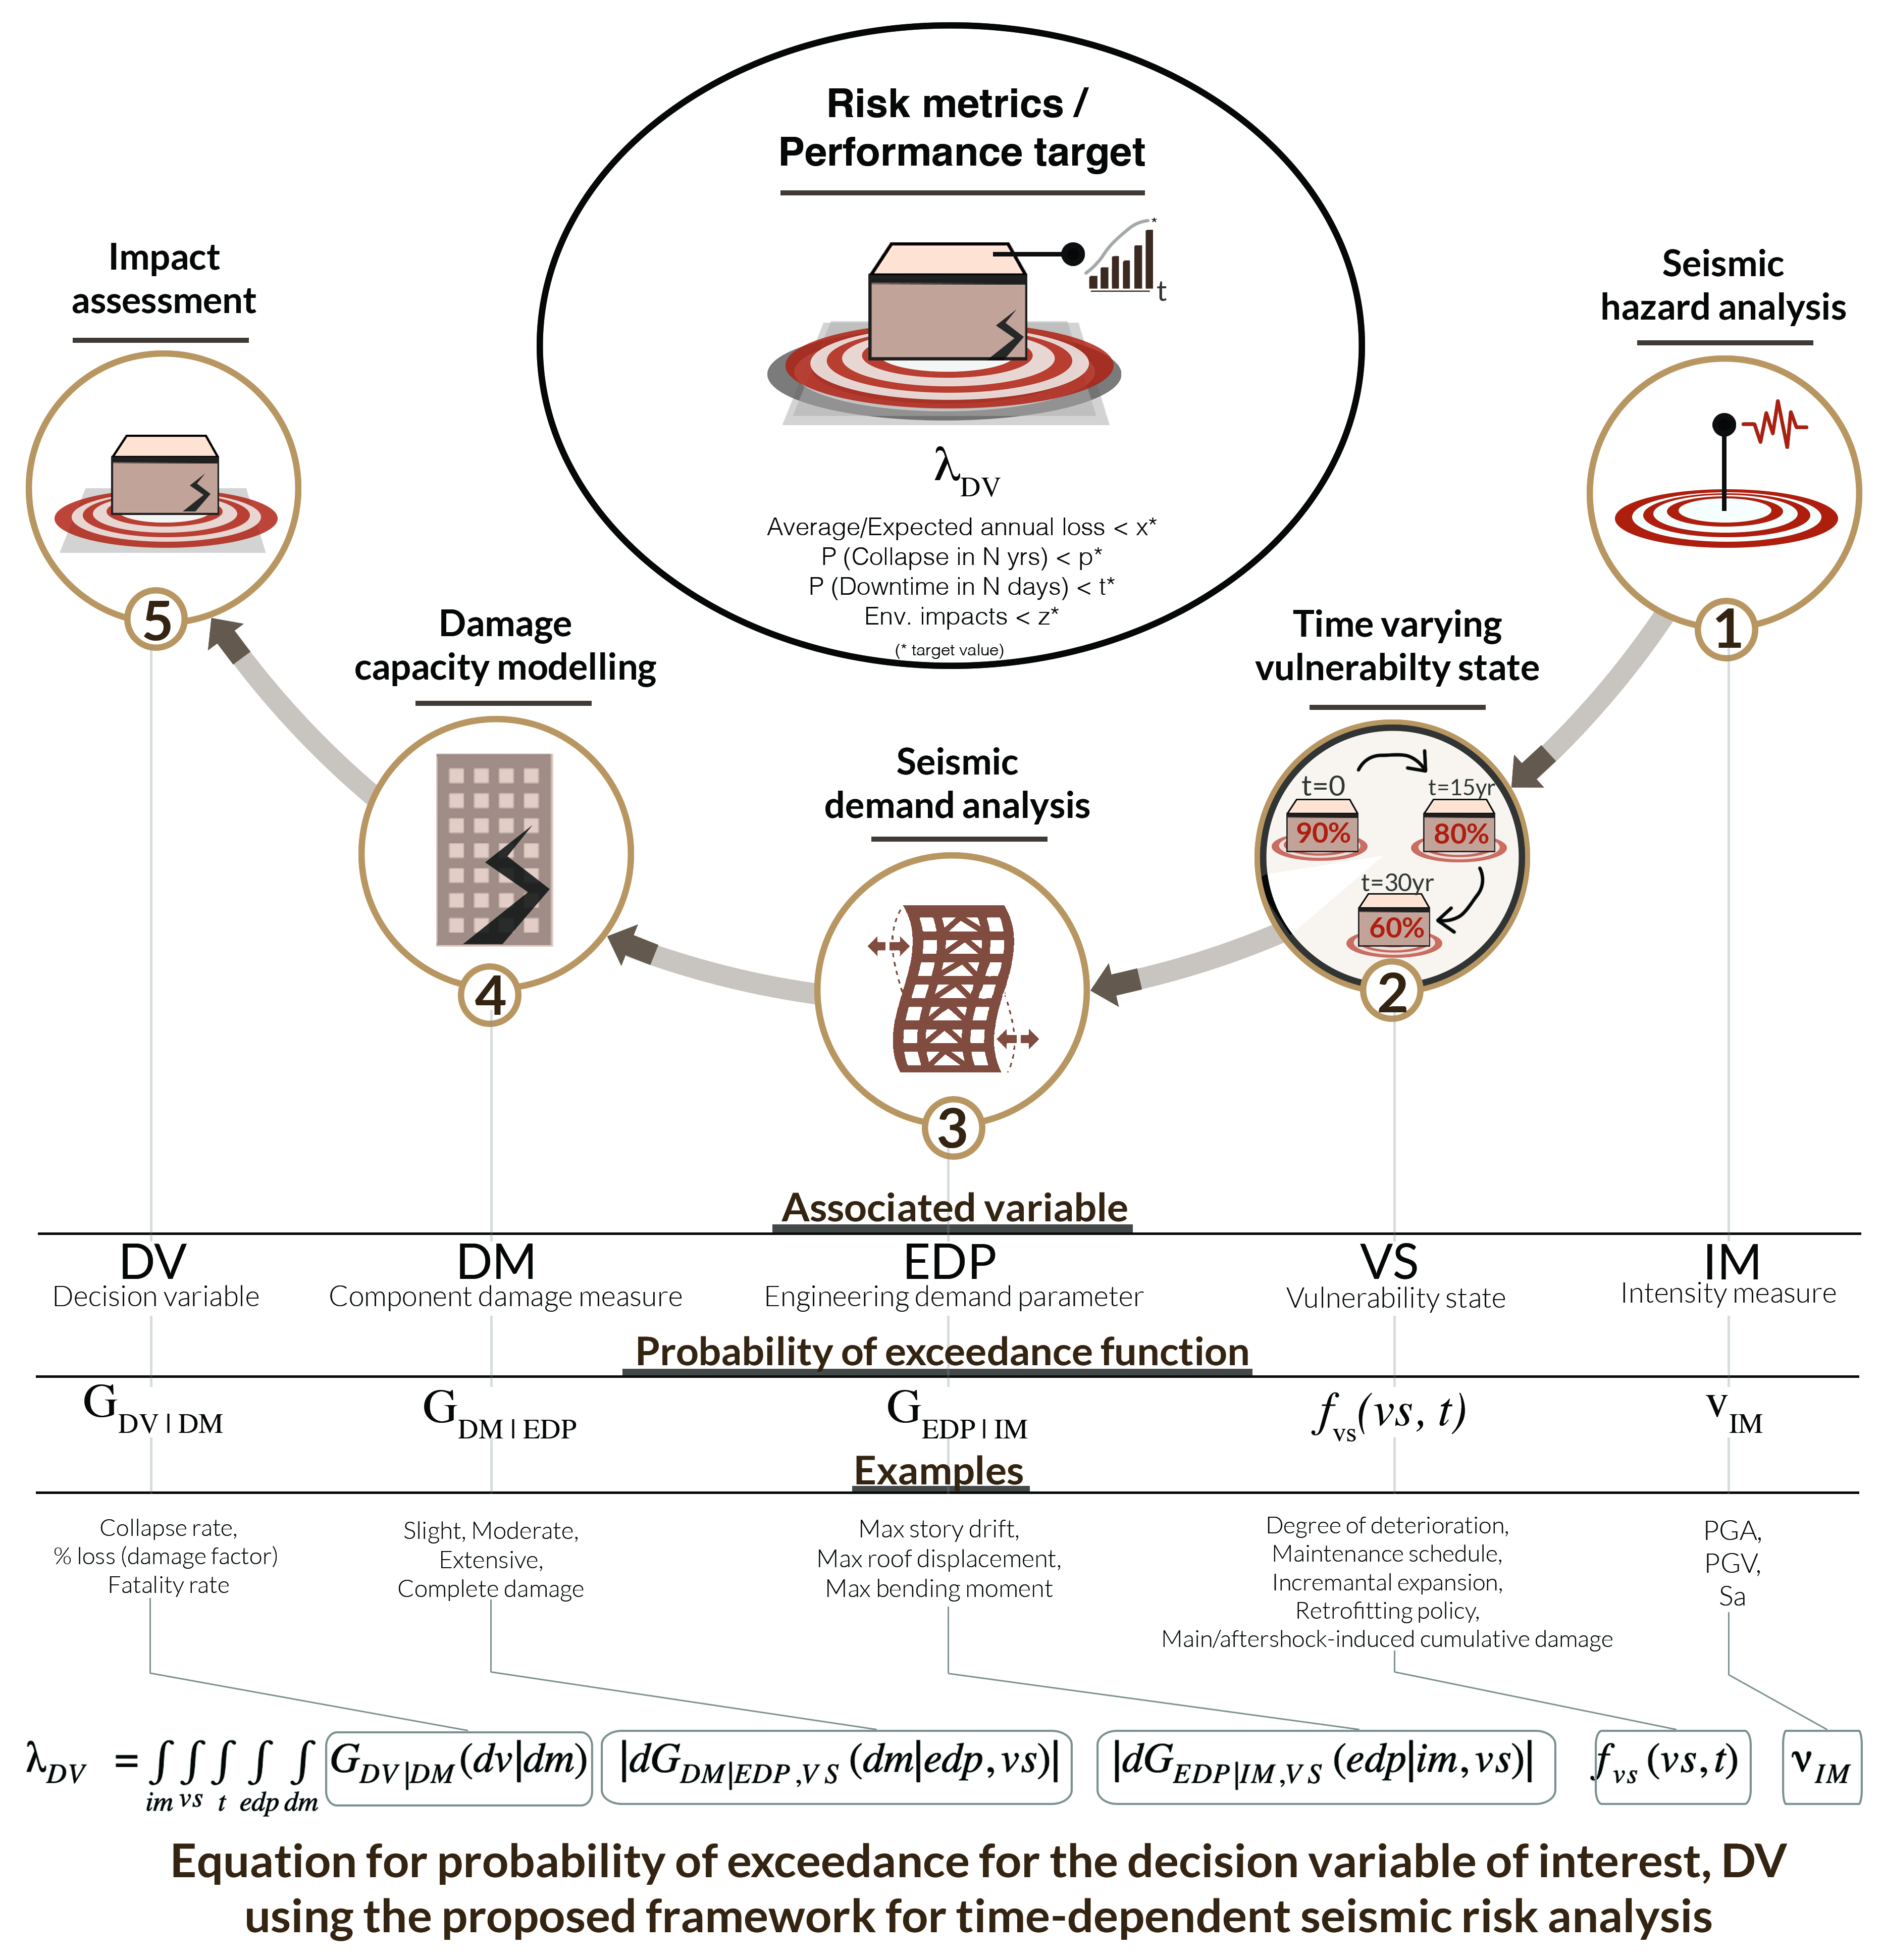
\includegraphics[width=\linewidth]{Figures/ICASP_Schematic1.jpg}
  \caption{Proposed framework accounting for time dependent vulnerability in seismic risk analysis}
  \label{fig:schematic1}
\end{figure*}  


\afterpage{%
    \clearpage% Flush earlier floats (otherwise order might not be correct)
    \begin{landscape}% Landscape page
\begin{figure*}[h!]
  \centering
  \includegraphics[width=\linewidth]{Figures/ICASP_Schematic2_matrix.jpg}
  \caption{Potential time-dependent vulnerability drivers for seismic risk and associated transition scenario}
  \label{fig:schematic2}
\end{figure*}  

\end{landscape}
\clearpage% Flush page
}

%% Discussion of transition

\subsection{Mathematical representation of vulnerability states and corresponding transition scenario}

Along with the proposed framework shown in Figure \ref{fig:schematic1}, we illustrate in Figure \ref{fig:schematic2} several potential time-dependent vulnerability drivers for seismic risk.

A certain vulnerability state can be dependent on the building's degree of deterioration, state of expansion, current structural condition, or the developed retrofit standard depending on the significant vulnerability drivers of interest to a certain structure. Given in Figure \ref{fig:schematic2} are suggested relative vulnerability states exhibiting increasing seismic vulnerability (for deterioration and building replacement) and decreasing vulnerability/increased resilience states (for seismic retrofitting).

Using Markov Chains is a simple approach to represent the transition of these discrete states over time. Markov chains are used to map the probability of transitioning from one state to another state in a specific time interval. Markov models are “memoryless”, such that the new state is solely dependent on the current state; not on the set of events preceding it \citep{agresti2003categorical}. The column showing the 'Transition Scenario' provides a schematic of the types of transition processes linked to each time-dependent vulnerability driver, and can then be mapped into corresponding transition probability matrices.

For instance, a non-retrofitted building can either transition into a retrofitted state with a certain probability within a year, or it can stay in its current state. Similarly, a building can also transition into a more deteriorated state over time with an associated transition probability. A common assumption for analysis incorporating structural deterioration or seismic retrofitting is that once a certain state is reached, it cannot go back to a previous state. For example, we assume that once a building is retrofitted, it is not possible for the building to go back to its unretrofitted state. In the schematic for the transition scenarios (Fig. \ref{fig:schematic2}) of deterioration and seismic retrofitting, this is shown by having all transition arrows going to the right only.
On the contrary, possible transition patterns for building replacements can bring back a building to its original (as-new) state as time goes by as presented by the arrows going to the left in its transition scenario diagram (Figure \ref{fig:schematic2}). Alternatively, a building could be replaced by another built to higher standards, as is often the case resulting from building code improvements. The same figure also shows a sample transition probability matrix for each vulnerability driver using the given time-dependent vulnerability states. The size of the transition probability matrix depends on the potential vulnerability states considered in the analysis, but they should exhibit similar pattern. 

Depending on the transition rates, $d_{i,i}$, $b_{i,i}$, $r_{i,i}$, the transition between the vulnerability states can go either slower or quicker based on different factors. For example, building deterioration rates are usually affected by the level of environmental exposure of the structure, its initial structural quality, or the implemented maintenance schedule which could potentially mitigate the seismic risk over time.
It should be noted that the factors affecting transition rates don't necessarily affect the actual fragility curve for each state.

Fragility curves define the state of vulnerability of a building or structure. These curves show the relationship of the earthquake intensity and the probability of exceeding a particular damage level.

Numerous methods exist to derive these curves: (1) analytical \citep{singhal1996method, lallemant2015statistical}, (2) empirical \citep{sanchez2005science,noh2015development} or heuristic/ based on expert opinion \citep{jaiswal2012use}.

Given a hazard curve at a study site, the annual collapse rate of a building is calculated by integrating the fragility curve over the hazard curve in Equation \ref{eq:onebldg}.
\begin{equation}
\begin{split}
    \lambda_{Collapse} = \Int_{IM_{min}}^{IM_{max}} P(Collapse |IM=im) | d\lambda_{im} (im) |
\end{split}
\label{eq:onebldg}
\end{equation}

where $\lambda_{im} (im)$ is the seismic hazard curve and $| d\lambda_{im} (im) |$ is the absolute value of the derivative of the hazard curve.

For a portfolio of buildings  the annual expected number of building collapse at a time $t$ can be calculated using Equation \ref{eq:port}.
%\begin{footnotesize}
%\begin{strip}
\begin{equation}
\begin{split}
    \lambda_{Collapse Total}(t) = \sum_{State_{1}}^{State_{n}}\Int_{IM_{min}}^{IM_{max}}\\
     P(Collapse |IM=im)| State=State_{i})  \\
     \times \; P(State=State_{i} |D_{o} =d_{o}, P=p)(t) \\
    \times \; | d\lambda_{IM} (im) |
\end{split}
\label{eq:port}
\end{equation}
%%\end{footnotesize}

where $P(Collapse |IM=im)| State=State_{i}$ is the fragility curve for each building state at collapse,  
$P(State=State_{i} |D_{o} =d_{o}, P=p)(t)$  is the probability of being in a building state at time $t$ for a given transition probability matrix $p$ and initial state distribution $d_{o}$.

It can be shown that the expected vulnerability state distribution $D_t$ at time $t$ is $E(D_t|D_o=d_o) = d_oP^t$ where $P$ is the transition probability matrix of vulnerability states. Therefore \ref{eq:port} can be re-written as:
\begin{equation}
\begin{split}
    \lambda_{Collapse Total}(t) = \sum_{State_{1}}^{State_{n}}\Int_{IM_{min}}^{IM_{max}}\\
    P(Collapse |IM=im)| State=State_{i}) \\
   \times \;  d_oP^t \; | d\lambda_{IM} (im) |
\end{split}
\label{eq:port2}
\end{equation}


\section{Case studies}

\subsection{Building-level deterioration analysis}

We apply the methodology discussed previously to model the changing risk of a hypothetical deteriorating building over time, we focus on three (3) vulnerability states ranging from as-new, heavily deteriorated and very heavily deteriorated for a hypothetical reinforced concrete (RC) building. 

A hypothetical vulnerability curve is generated to represent the non-deteriorated state. For simplicity, we only use fragility curves corresponding to "Extensive/ Complete Damage.”

Vulnerability curves for the three (3) assumed vulnerability states corresponding to each degree of deterioration,$w$, are obtained using Equations \ref{eq:rao1} and \ref{eq:rao2} \citep{rao2017development}. 
\begin{equation}
\begin{split}
    m(w) = m_{o}e^{-\alpha_{m}w}
\end{split}
\label{eq:rao1}
\end{equation}
\begin{equation}
\begin{split}
    \xi(w) = \xi_{o}(1-\alpha_{\xi}w)
\end{split}
\label{eq:rao2}
\end{equation}

where \\
$m(w)$, $\xi(w)$= median and dispersion of fragility function at level of deterioration $w$ consecutively ,\\
%$\xi(w)$= dispersion of the fragility function at a level of deterioration $w$, \\
$m_{o}$, $\xi_{o}$ = median and dispersion of the fragility function for the column in its non-corroded state consecutively\\
%$\xi_{o}$=  dispersion of the fragility function for the column in its non-corroded state, \\
$\alpha_{m}$=  exponential decrement function for the median and \\
$\alpha_{\xi}$=  coefficient of the linear decrement function for the dispersion of the fragility function.

The coefficients of the decrement function are adopted from estimates by \cite{rao2017development} for a hypothetical RC column built in 1960 to pre-1971 design standards: 
$m=1.43$,	$\alpha_{\xi}= -0.18 $

Using the framework for this application, we compare the impact of different levels of maintenance on seismic risk over time. Three maintenance schemes are used to demonstrate the diversity of maintenance options for seismic safety: (1) Low, (2) Medium, and (3) High Maintenance.
Transition probability matrices are assumed based on a Markovian model developed by Duling (2006) for an RC building constructed with pre-1971 design standards to predict the building service life given three varying levels of maintenance. The percent change in annual collapse risk normalized to baseline risk at t=0 is calculated using Equation \ref{eq:onebldg} and presented in Figure \ref{fig:bldglevel}. 

The trends shown in the figure highlight the impact of building deterioration on the seismic risk of buildings, and the benefits of maintenance; it demonstrates the importance of accounting for time-dependent vulnerability drivers such as deterioration in studying future seismic risk of a building. This demonstration shows that the proposed framework enables the testing of impact of maintenance or other building mitigation strategies on seismic risk over time. If linked with financial loss information, the framework could be used for cost benefit analysis for mitigation.

\begin{figure}[htbp!]
  \centering
  \includegraphics[width=\linewidth]{Figures/building_level.png}
  \caption{Percent change in annual collapse risk normalized to baseline risk at t=0 for a hypothetical building}
  \label{fig:bldglevel}
\end{figure}  

%%% DISCUSSION

%% Building levels
%% The framework demonstrates how we can investigate changing vulnerability over time driven by these factors
%% Buildings deteriorate over time even with high level of maintenance - this needs to be accounted for
%% It also enables to test impact maintenance or other building mitigation strategies
%% If linked with, financial loss, it could be used for cost benefit analysis for mitigation

%%%%%%%%%%%%%%%%%

\subsection{Policy analysis for community level seismic risk reduction}


%%%% Seismic Risk Reduction Policies


Using the proposed framework, we can also test the impact of various seismic risk reduction policies at a regional level. A hypothetical urban community was simulated, consisting of four districts each having their own building type distribution and seismic hazard curve. For simplicity of demonstration, the design of buildings are either high grade or low grade, and each can transition to deteriorated states, retrofitted states (for low-grade buildings), or get replaced over time. Hypothetical fragility curves are developed to represent each of these states: (1) Undeteriorated/unretrofitted state (2) Heavily deteriorated state (3) Very heavily deteriorated state (4) Retrofitted state with low standard and (5) Retrofitted state with high standard. The fragility curves for each vulnerability state are shown in figure \ref{fig:fragcurves}.

Hazard curves for each district are synthetically generated as idealized power-law hazard curves of the following form:
\begin{equation}
\begin{split}
    \lambda_{im} (IM) = k_{o}IM^{-k}
\end{split}
\label{eq:rao2}
\end{equation}

Parameters used for the four districts are k0 = 0.0002, 0.0003, 0.00022, 0.00035 and k = 2, 2.1, 2.2, 2.5
for districts 1, 2, 3 and 4 respectively.

%%Maybe insert plot of fragility curves

\begin{figure}[htbp!]
 \centering
  \includegraphics[width=.7\linewidth]{Figures/fragcurves5.jpg}
  \caption{Fragility curves for assumed vulnerability states at the hypothetical building stock}
  \label{fig:fragcurves}
\end{figure} 

% Please add the following required packages to your document preamble:
% \usepackage{booktabs}


\begin{table}[]
\centering
\caption{Indices of Transition Probability Matrices. (Abbreviations: HD = Heavily deteriorated, VHD = Very heavily deteriorated, n/a = Unretrofitted building}
\begin{tabular}{@{}lllllllll@{}}
\toprule
Index                                                             & P1     & P2   & P3   & P4     & P5  & P6  & P7     & P8     \\ \midrule
\begin{tabular}[c]{@{}l@{}}Building\\ design grade\end{tabular}   & high   & high & high & low    & low & low & any    & any    \\ \midrule
\begin{tabular}[c]{@{}l@{}}Degree of\\ deterioration\end{tabular} & as-new & HD   & VHD  & as-new & HD  & VHD & as-new & as-new \\ \midrule
\begin{tabular}[c]{@{}l@{}}Retrofit\\ standard\end{tabular}       & n/a    & n/a  & n/a  & n/a    & n/a & n/a & low    & high   \\ \bottomrule
\end{tabular}
\label{tab:mat}
\end{table}


%\begin{figure}[htbp!]
 %\centering
 % \includegraphics[width=5cm]{Images/trans_format.jpg}
 % \caption{Form of transition probability matrix for the community level policy analysis. Refer to Table \ref{tab:mat} for description of each state.}
 % \label{fig:transformat}
%\end{figure} 

\begin{figure}[htbp!]
 \centering
  \includegraphics[width=.7\linewidth]{Figures/trans_low.jpg}
  \caption{Transition probability matrix calibrated for a low quality seismic risk reduction scheme described in Table \ref{tab:policylist}}
  \label{fig:transprob1}
\end{figure} 

\begin{figure}[htbp!]
 \centering
  \includegraphics[width=.7\linewidth]{Figures/trans_high.jpg}
  \caption{Transition probability matrix calibrated for a high quality seismic risk reduction scheme described in Table \ref{tab:policylist}}
  \label{fig:transprob2}
\end{figure} 



The purpose of the framework developed is to compare the impact of
various policies on seismic risk over time. The types of decisions in the policy-making space includes the level of retrofit standards used, maintenance schedule and rate of development (building replacement) in each district. All these are being implemented while taking into account deterioration rate. Mathematically, the transition matrix for this type of problem is represented by a combination of the typical transition probability matrices shown in Figure \ref{fig:schematic2}. Two community-level policies are simulated using the proposed framework as described in Table \ref{tab:policylist}. Corresponding transition probability matrices for each policy are shown in Figures \ref{fig:transprob1} and \ref{fig:transprob2}. Each value corresponds to the probability of each state described in Table \ref{tab:mat} to  transition to the next state.

\afterpage{%
    \clearpage% Flush earlier floats (otherwise order might not be correct)
    \begin{landscape}% Landscape page
% Please add the following required packages to your document preamble:
% \usepackage{booktabs}
% \begin{tiny}
\begin{table*}[]
\centering
% \footnotesize
\caption{Features of seismic reduction policies tested on a hypothetical community}
\begin{tabular}{@{}lll@{}}
\toprule
Policy feature              & Low quality seismic reduction scheme                        & High quality Seismic reduction scheme                         \\ \midrule
Retrofit policy             & Voluntary, long time frame, low standard & Mandatory, short time frame, high standard \\
Building replacement policy & Low rate of replacement                                     & High rate of replacement                                      \\
Maintenance schedule        & Low level maintenance schedule                              & High level maintenance schedule \\\bottomrule                             
\end{tabular}
\label{tab:policylist}
\end{table*}
% \end{tiny}
\end{landscape}
\clearpage% Flush page
}

Using Equation \ref{eq:port}, the change in risk linked to these two policies implemented on the hypothetical building stock is demonstrated in Figure \ref{fig:commlevel}. As expected, mandatory retrofit schemes with shorter time frames result in early and rapid reduction in seismic risk (Figure \ref{fig:commlevel}). Also, better maintenance schedules significantly slow down the deterioration of a building portfolio thus reducing seismic risk over time. Demonstrated in the hypothetical building stock case as well is that encouraging development or high building replacement rates to better code standards contributes to seismic risk reduction over time. This demonstration of a policy analysis for community level seismic risk reduction demonstrates the capability of the proposed framework to compare various policy choices related to different standard of improvements such as building codes or time frame for which these policies are enforced/implemented.

Note that the framework can be used to test complex combinations of policies, including encouraging development in lower-hazard districts, different retrofit time-frames, retrofit standards, new building codes, and much more.

\begin{figure}[htbp!]
  \centering
  \includegraphics[width=\linewidth]{Figures/community_level.png}
  \caption{Percent change in annual collapse risk normalized to baseline risk at t=0 for a hypothetical building stock. Refer to Table \ref{tab:policylist} for descriptions of each policy }
  \label{fig:commlevel}
\end{figure} 

% Community level
%%% Add another policy (middle curve?)
%% Demonstrates time dependent risk community scale driven by all these facotrs
%enables comparison of various ppolicy choices both related to standard of imprpovemnets - building codes, time frame for which policies are enforced/implemented


\section{Conclusion}

This paper presents a flexible framework accounting for time dependent vulnerability in seismic risk analysis. 
This enables modelling both of those processes that increase vulnerability (e.g.deterioration, building expansions, cumulative damage), those policies that mitigate increase in vulnerability (e.g. better maintenance schedule, higher durability construction) and those policies that improve resilience (e.g. seismic retrofits and building replacement to higher standards).

We provided multiple applications of the proposed framework for risk analysis that accounts for time-dependent vulnerability. We demonstrated a building-level deterioration analysis and a community-level seismic risk reduction policy analysis. The applications vary in terms of the modelled drivers of changing vulnerability and the scale of application (building-level vs. community-scale). In Appendix \ref{app-time-paper}, I include a short paper that demonstrates a variation of the flexible community-scale analysis shown in this chapter. The application focuses on testing seismic retrofitting programs with varying levels of retrofit standard, time-frame of implementation and whether the program is mandatory or voluntary. The case study in Appendix \ref{app-time-paper} uses fragility data and transition probabilities derived from New Zealand's seismic retrofit implementation records. This example further highlights the potential and flexibility of the time-dependent risk framework presented in this chapter to evaluate specific risk interventions.

Overall, the methodology builds on the fundamental probabilistic performance based framework by adding a component for time-varying features which affect vulnerability. The framework allows stakeholders to study the consequences of different mitigation schemes to future seismic risk, and analyse its sensitivity to the initial building stock quality, the structural deterioration rate, maintenance schedule, features of mandatory retrofit policies in terms of their time-frame and standard, building replacement rate, urban development rates and pattern, and other drivers of changing risk.


%----------------
\section{Acknowledgments}
%----------------
This research is funded through a National Research Foundation (Singapore) Fellowship grant (NRF–NRFF2018–06), along with an Earth Observatory of Singapore scholarship.


%The current demonstration is simplified.. 
% LImitattion

%%% Change module --> component
%% 
